\documentclass{amsart}
\usepackage{fullpage}

\usepackage[T1]{fontenc}
\usepackage[utf8]{inputenc} 
\usepackage{lmodern}
\usepackage[slovene]{babel}
\usepackage{amsmath,amssymb,amsfonts}
\usepackage{bbm}
\usepackage{graphicx}
\graphicspath{{./images/}}

\linespread{1.2}

\newcommand{\N}{\mathbb{N}}
\newcommand{\Z}{\mathbb{Z}}
\newcommand{\Q}{\mathbb{Q}}
\newcommand{\R}{\mathbb{R}}
\newcommand{\C}{\mathbb{C}}

% ukazi za matematicna okolja
\theoremstyle{definition} % tekst napisan pokoncno
\newtheorem{definicija}{Definicija}[section]
\newtheorem{primer}[definicija]{Primer}
\newtheorem{opomba}[definicija]{Opomba}

\renewcommand\endprimer{\hfill$\diamondsuit$}


\theoremstyle{plain} % tekst napisan posevno
\newtheorem{lema}[definicija]{Lema}
\newtheorem{izrek}[definicija]{Izrek}
\newtheorem{trditev}[definicija]{Trditev}
\newtheorem{posledica}[definicija]{Posledica}

\title{Kontekstno-neodvisne gramatike za kodiranje in stiskanje podatkov}
\author{Janez Podlogar}
\date{\today}

\begin{document}

\begin{abstract}

    V delu predstavimo motivacijo in osnovne pojme, ki so potrebni za obravnavnje
    stiskanja podatkov s kontekstno-neodvisnimi gramatikami.

\end{abstract}

\maketitle

\section{Kodiranje podatkov}

Zapis informacije v neki obliki ni primeren za vsakršno rabo. Besedilo, zapisano z 
pismenkami, je neberljivo za slepe osebe, saj je komunikacijski kanal v tem primeru
vid. Prav tako pisanega besedila v pravotni obliki ni moč poslati z telegrafom. V tem
primeru je komunikacijski kanal žica in pismenke se po njej ne morejo sprehoditi. V obeh 
primerih je informacija, ki bi jo radi prenesli v neprimerni obliki. V prvem 
primeru je potrebno besedilo zapisati z Braillovo pisavo. V drugem primeru pa je 
potrebno besedil pretvoriti v električni signal. Spreminjanje zapisa sporočila
pravimo \textit{kodiranje}, sistemu pravil, po katerem se kodiranje opravi,
pa \textit{kod}. 

\begin{primer}

    \textit{Morsejeva abeceda} je kodiranje črk, števil in ločil s pomočjo zaporedja kratkih
    in dolgih signalov:

    \begin{itemize}
        \item Dolžina kratkega signala je ena enota.
        \item Dolgi signal je trikrat daljši od kratkega signala.
        \item Razmiki med signali znotraj znaka so dolžine kratkega signala.
        \item Presledki med znaki so dolgi tri kratke signale oz. en dolgi signal.
        \item Presledki med besedami so dolgi sedem kratkih signalov.
    \end{itemize}

    \begin{figure}[h]
        \centering
        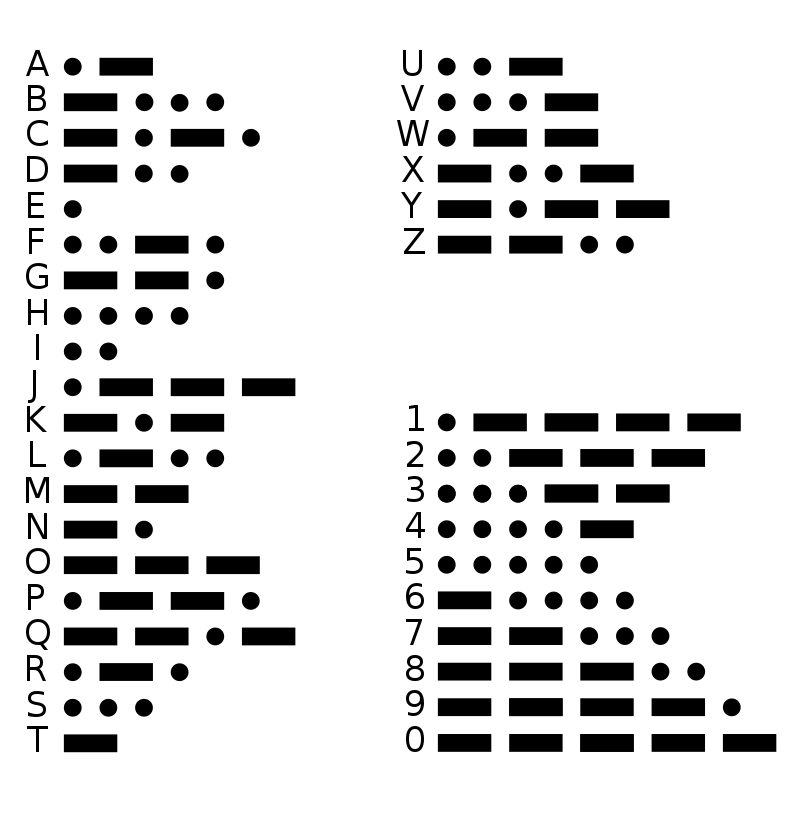
\includegraphics[width=4.3cm]{International_Morse_Code.svg.png}
        \caption{Mednarodna Morsejeva abeceda}
    \end{figure}

    Prvotni namen Morsejeve abecede je komunikacija preko telegrama, saj komunikacijski
    kanal dovoljuje le električne signale in tišino med njimi.  Kodiranje črk je takšno,
    da imajo črke z višjo frekvenco (v angleškem jeziku) krajši zapis, s tem se dolžina
     kodiranega sporočila skrajša in posledično tudi čas prenosa.

\end{primer}

\begin{definicija}

    \textit{Abeceda} je vsaka neprazna množica $ \Sigma $. \textit{Množica vseh besed na    % beseda zamanjati za niz
    abecedi} $ \Sigma $ je:

    \begin{equation*}
        \Sigma^* = \{ \, a_1 a_2 a_3 \dots \mid \forall i: a_i \in \Sigma \, \} \cup \{ \varepsilon \}, 
        % Bi bilo morda bolje definirati takole:
        % \Sigma^* = \{ \, a_1 a_2 a_3 \dots a_n \mid \forall i: a_i \in \Sigma \, \} \cup \{ \varepsilon \}
    \end{equation*}

    kjer $ \varepsilon $ prazna beseda.

\end{definicija}

V splošnem ima lahko abeceda poljubno kardinalnost, v diplomski nalogi se bomo srečali le z končnimi abecedami.
% Kaj se tukaj zgodi z 

\begin{primer}
    
    Naj bo $ \Sigma = \{ a,b,c \} $ abeceda, potem je:

    \begin{align*}
        ab \in \Sigma^* \\
        ccc \in \Sigma^* \\
        cababcccababcccab \in \Sigma^*
    \end{align*}

\end{primer}

\section{Kompresija podatkov}

\section{Kontekstno-neodvisne gramatike}

\end{document} 